 %%
 % COMAP2024SCUT template
 % Created by Caibin Zeng, email: macbzeng@scut.edu.cn  %
 % January 8, 2025
 %%
 
 %美赛模板:正文部分

 \documentclass[12pt]{article}  % 官方要求字号不小于 12 号,此处选择 12 号字体
 % \linespread{1.1}
 % \bibliographystyle{plain}
 % 本模板不需要填写年份,以当前电脑时间自动生成
 %%%%%%%%%%%%%%%%%%%%%%%%%%%%%%%%%%%%%%%%%%%%%%%%%%%%%%%%%%%%%%%%%%%%%%%%%%%%%%%
 % 请在以下的方括号中填写队伍控制号
 \usepackage[2511654]{easymcm}  % 载入 EasyMCM 模板文件
 \problem{B}  % 请在此处填写题号
 %%%%%%%%%%%%%%%%%%%%%%%%%%%%%%%%%%%%%%%%%%%%%%%%%%%%%%%%%%%%%%%%%%%%%%%%%%%%%%%%
 % \usepackage{mathptmx}  % 这是 Times 字体,中规中矩 
 \usepackage{palatino}  % mathpazo 这palatino是 COMAP 官方杂志采用的更好看的 Palatino 字体,可替代以上的 mathptmx 宏包
 \usepackage{pdfpages}
 \usepackage{longtable}
 \usepackage{tabu}
 \usepackage{threeparttable}
 \usepackage{listings}
 \usepackage{paralist}
 \usepackage{hyperref}
 \usepackage[linesnumbered,ruled,vlined]{algorithm2e}
 \usepackage{subfigure}
 \usepackage{subcaption}
 \usepackage{cleveref} %可以调用
 \usepackage{tcolorbox}
 \tcbuselibrary{most}
 \newtcolorbox{mybox}[2][]{colbacktitle=red!10!white, colback=blue!10!white,coltitle=red!70!black, title={#2},fonttitle=\bfseries,#1}
 \graphicspath{{img/}}          % 此处{img/}为相对路径,注意加上“/”
  \let\itemize\compactitem
  \let\enditemize\endcompactitem
 \newcommand{\upcite}[1]{\textsuperscript{\textsuperscript{\cite{#1}}}}
 
 
 \title{The Title Should be Concise and Informative}  % 标题
 
 % 如需要修改题头(默认为 MCM/ICM),请使用以下命令(此处修改为 MCM)
 %\renewcommand{\contest}{MCM}
 
  %文档开始
 \begin{document}
 
 % 此处填写摘要内容
 \begin{abstract}
Juneau City in Alaska, USA is facing the problem of overtourism. The number of tourists and tax rates need to be adjusted to improve the satisfaction of tourists and residents, and finally realize sustainable development of tourism industry. The government has implemented some measures to limit the number of tourists, protect the environment, and improve local infrastructure, but the results have not been satisfactory due to the complex factors affecting tourist and resident satisfaction.
     
This article establishes a new satisfaction evaluation model that comprehensively considers the impact of tourist numbers on residents' income, government spending, ecological environment, and social pressure, in order to adjust the daily number of tourists and achieve multi-objective optimization of tourist and resident satisfaction.

\textit{The main steps are as follows:}
 
First, a causal model was established to analyze the principle of how the number of tourists affects tourist satisfaction and resident satisfaction.

 Then, based on the causal model and combined with the searched data, several equations were established to construct a multi-objective optimization model for the impact of tourist numbers on tourist satisfaction and resident satisfaction.

 To maximize stakeholder satisfaction, the NSGA-II genetic algorithm is used to solve the Pareto solution of the multi-objective problem and determine the optimal number of tourists.
 
 This study successfully simulated and optimized the number of tourists in Juneau city by constructing a causal diagram model, which benefits both tourists and residents, and more importantly, can achieve sustainable development of tourism in the Juneau area. In addition, through adjustments, the model can be applied to other destinations affected by excessive tourism and has good universality.
     
 % 此处填写关键字,以分号分开
     \vspace{5pt}  %mm	毫米	1 mm = 2.845 pt   pt 点	1 pt = 0.351 mm
     \textbf{Keywords}: Causal Model; Overtourism; Multi-objective optimization; NSGA-II; Sustainable tourism;
 
 \end{abstract}
 
 \maketitle  % 生成 Summary Sheet
 
 \tableofcontents  % 生成目录
 
 
 % 正文开始
 % Chapter 1: Introduction
 \section{Introduction}
 \subsection{Background}
In recent years, the rapid development of the global tourism industry has brought many challenges, among which the problem of overtourism is particularly prominent. Take Juneau, Alaska, USA as an example. The city received about 1.6 million cruise passengers in 2023, setting a new record. On the busiest days of the tourism season, Juneau could receive up to seven large cruise ships, with as many as 20,000 visitors. Although these tourists brought in a substantial revenue of about 375 million dollars for the city, they also caused many problems, such as increased pressure on local infrastructure, tight drinking water supply, difficult waste management, and increased carbon footprint. In addition, overtourism has also had a negative impact on local culture and natural landscapes, of which the recession of Mendenhall Glacier is a typical case. Since 2007, the glacier has receded the equivalent of eight football fields, which not only caused local residents to worry about the disappearance of the glacier, but also raised questions about the sustainability of tourism. Therefore, how to maintain the economic benefits of tourism while reducing its negative impact on the environment and society, and achieve sustainable development, has become an urgent problem for Juneau to solve.
 
 \subsection{Restatement of the Problem}
 Given the context of overtourism in Juneau, Alaska, and its implications on both the environment and local community, the following issues need to be addressed:
 \begin{itemize}
    \item[$\bullet$]Develop a sustainable tourism model for Juneau, considering factors such as visitor numbers, overall revenue, and tourism stabilization measures. Clearly identify the factors to be optimized and those serving as constraints. Include a financial plan for additional revenue and demonstrate its feedback loop into the model for sustainable tourism promotion. Conduct a sensitivity analysis to highlight the most critical factors.
    \item[$\bullet$]Adapt the model to other overtourism-affected destinations, considering how location choice impacts the importance of different measures. Explore ways to use the model to promote less-visited attractions or locations to achieve a balanced tourism distribution.
    \item[$\bullet$]Draft a one-page memo to the Juneau Tourist Council, outlining predictions, the effects of various measures, and recommendations for optimizing outcomes.
 \end{itemize}
\subsection{Our Work}
 
To visually demonstrate our workflow, the flow chart is shown as Figure \ref{fig1}.
  
 
 
 \begin{figure}[H]  %h此处,t页顶,b页底,p独立一页,浮动体出现的位置 [H]
 
 \centering  %图表居中
 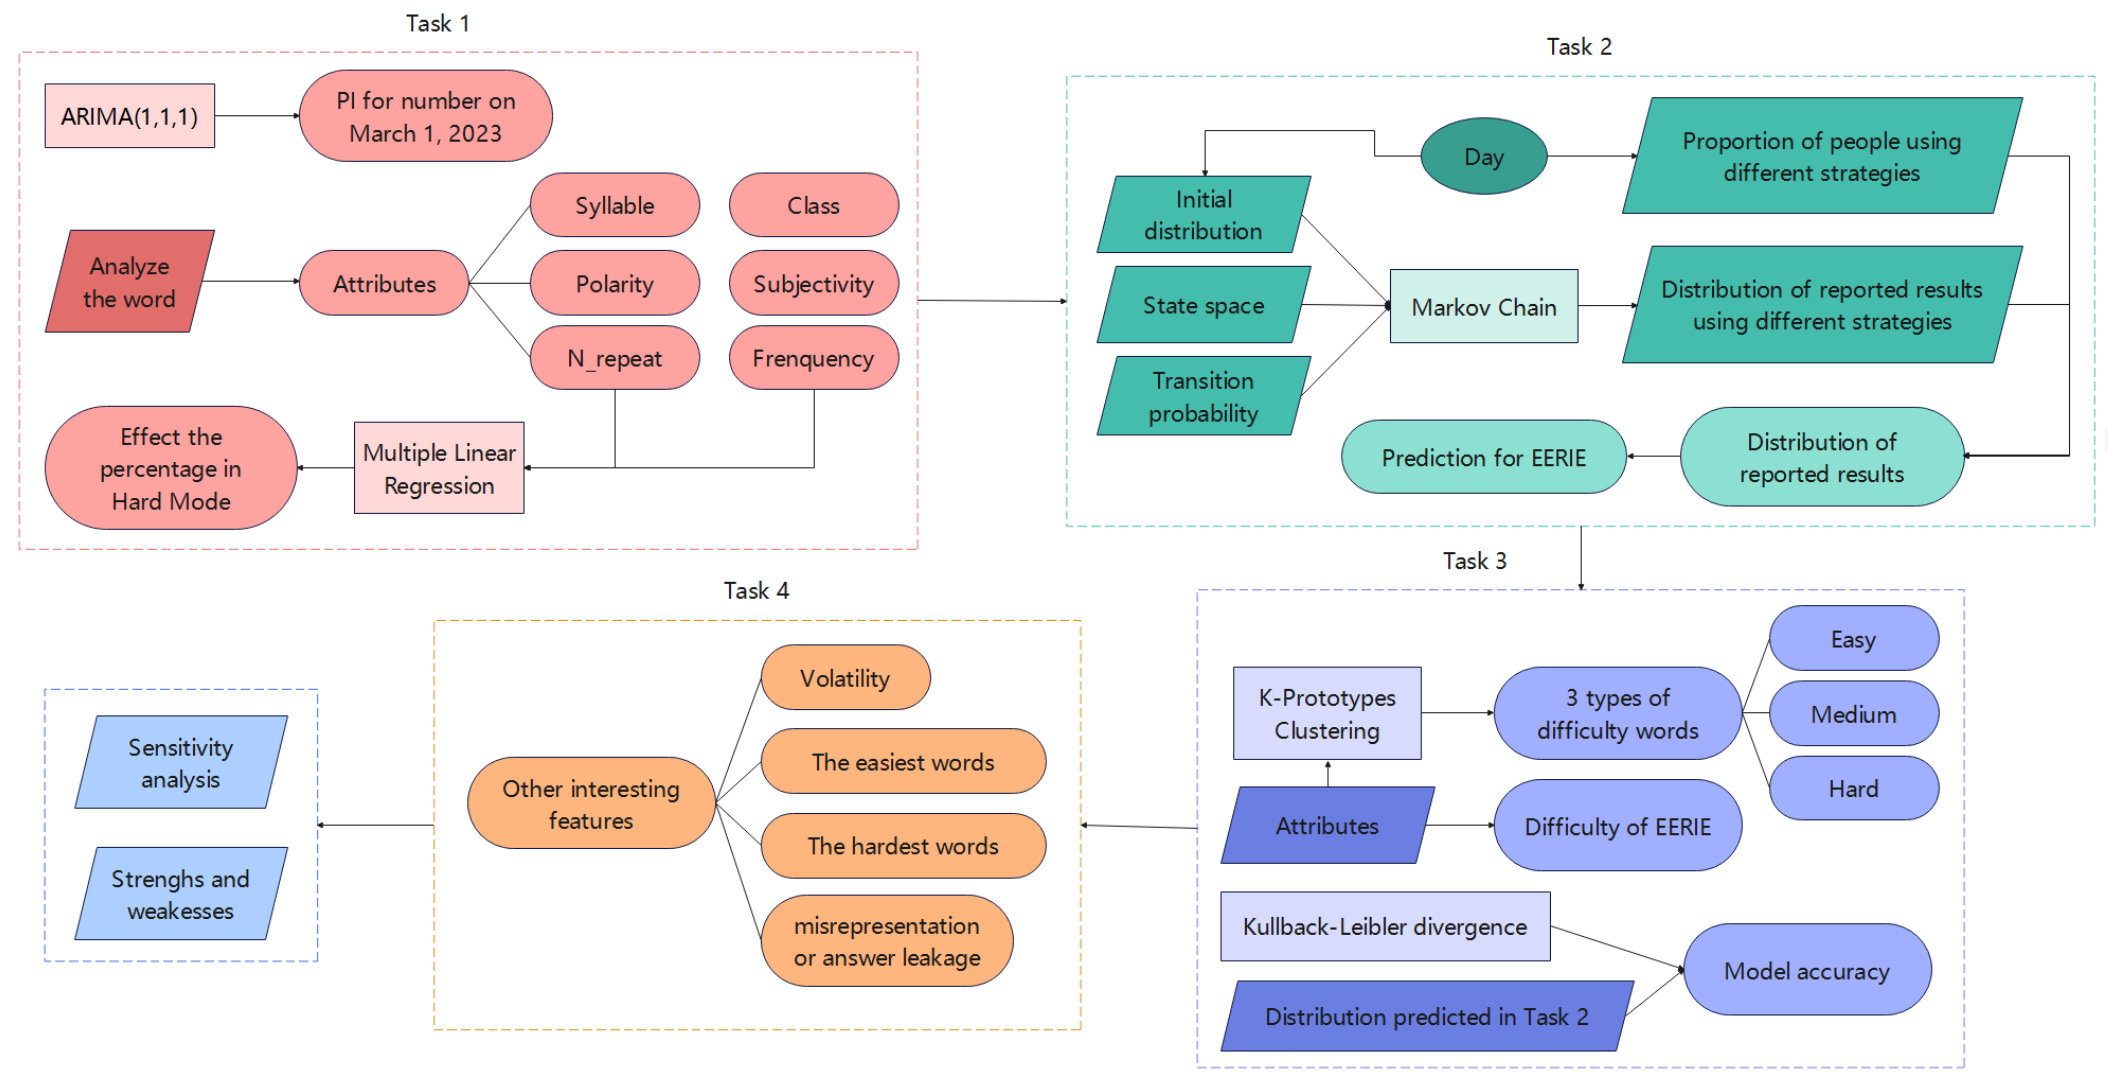
\includegraphics[width=.9\textwidth]{Flow_Chart.png} %图片的名称或者路径之中有空格会出问题 
 \caption{Flow Chart of Our Work (From Team \# 2318982)} % 图片标题 
 \label{fig1}%交互引用
 \end{figure}
 
 
 \section{Assumptions and Explanations}
 
 In this section, we need to make reasonable assumptions to simplify the problem and facilitate the modelling, and each hypothesis is closely followed by its appropriate explanation.
 
 \begin{itemize}
     \setlength{\parsep}{0ex} %段落间距
     \setlength{\topsep}{2ex} %列表到上下文的垂直距离
     \setlength{\itemsep}{1ex} %条目间距
     \item[\bfseries \textit{Assumption} 1:]  XXX
     \item[\bfseries \textit{Explanation:}]  XXX
     \vspace{1ex}
     \item[\bfseries \textit{Assumption} 2:]  XXX
     \item[\bfseries \textit{Explanation:}]  XXX
     \vspace{1ex}
         \item[\bfseries \textit{Assumption} 3:]  XXX
     \item[\bfseries \textit{Explanation:}]  XXX
 \end{itemize}
 
 Additional assumptions are made to simplify the analysis for individual sections. These assumptions will be discussed at the appropriate locations.
 
 \section{Notations}
 Some important mathematical notations used in this paper are listed in Table \ref{tab1}. 
 \begin{table}[htbp]
 \begin{center}
 \caption{Notations used in this paper}
 \begin{tabular}{cl} % 第一列居中对齐、第二列居左对齐
 \toprule[2pt]
 \multicolumn{1}{m{4cm}}{\centering Symbol}
 &\multicolumn{1}{m{10cm}}{\centering Description }\\  %3cm 和 8cm 是列宽,根据实际需求修改
 \midrule
 $x_i$   & XXXXX \\
 $y_i$   & YYYYYY \\
 \bottomrule[2pt]
 \end{tabular}	\label{tab1} % 交互引用 
  \begin{tablenotes}
         \footnotesize
         \item[*] *\href{https://www.caam.rice.edu/~heinken/latex/symbols.pdf}{ \LaTeX~Mathematical symbols collected by Prof. M. Heinkenschloss}. %此处加入注释*信息
       \end{tablenotes}
 \end{center}
 \end{table} 
 \vspace{-1cm} 
 
 
 
 \section{Data Preprocessing}
 
 This section is optional and the following texts are extracted from MonkeyLearn Blog \cite{Mesevage2021}. Data preprocessing is a step in the data mining and data analysis process that takes raw data and transforms it into a format that can be understood and analyzed by computers and machine learning.
 
 Raw, real-world data in the form of text, images, video, etc., is messy. Not only may it contain errors and inconsistencies, but it is often incomplete, and doesn’t have a regular, uniform design.
 
 So calculating structured data, like whole numbers and percentages is easy. However, unstructured data, in the form of text and images must first be cleaned and formatted before analysis.
 
 Depending on your data gathering techniques and sources, you may end up with data that’s out of range or includes an incorrect feature, like household income below zero or an image from a set of “zoo animals” that is actually a tree. Your set could have missing values or fields. Or text data, for example, will often have misspelled words and irrelevant symbols, URLs, etc.
 
 \begin{figure}[htbp]  %h此处,t页顶,b页底,p独立一页,浮动体出现的位置
     
     \centering  %图表居中
     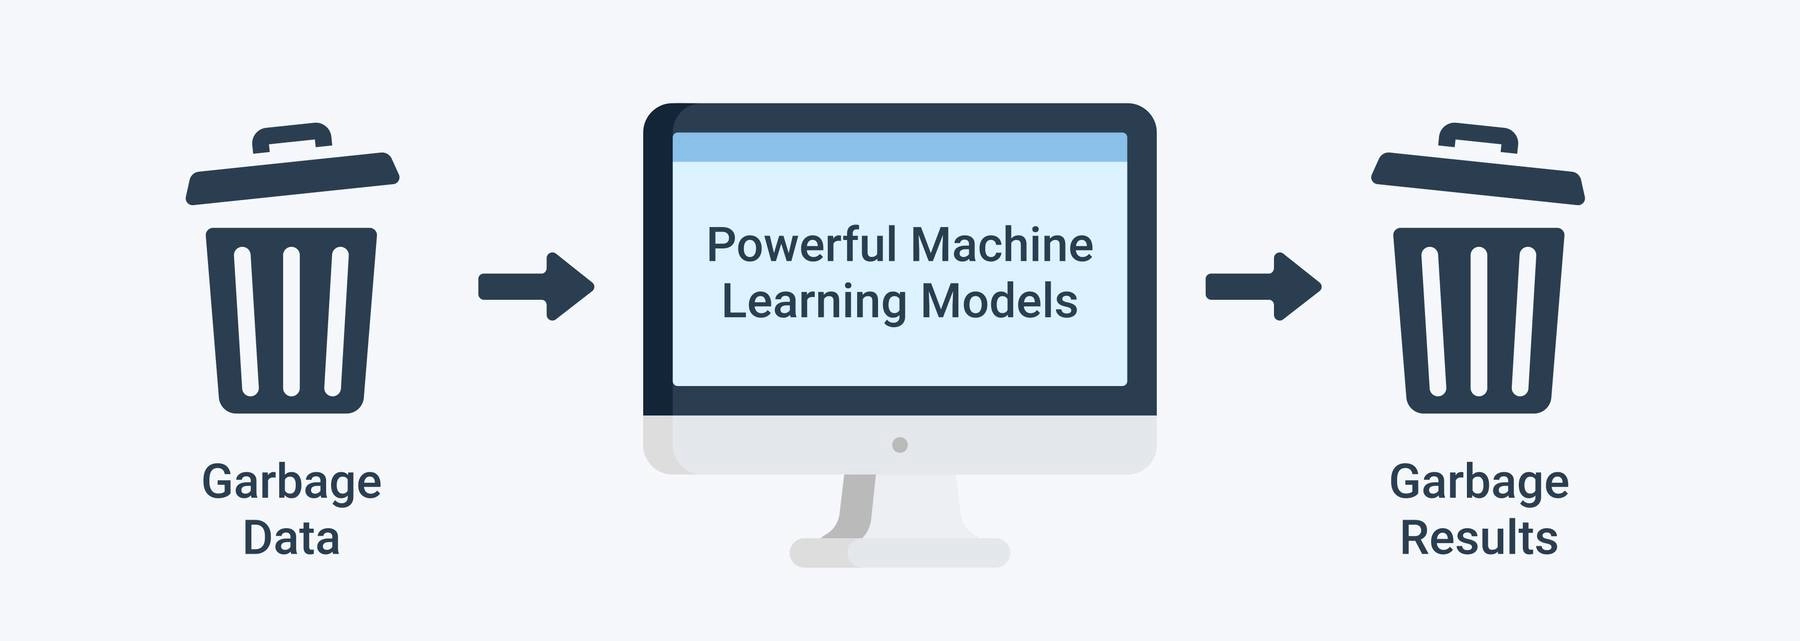
\includegraphics[width=.7\textwidth]{DataProc.jpg} %图片的名称或者路径之中有空格会出问题 
     \caption{Why data preprocessing is importance? (From MonkeyLearn Blog)} % 图片标题 
     \label{fig2}%交互引用
 \end{figure}
  
 
 Data sets can be explained with or communicated as the features that make them up. This can be by size, location, age, time, color, etc. Features appear as columns in datasets and are also known as attributes, variables, fields, and characteristics. 
 
 It’s important to understand what features are when preprocessing your data because you’ll need to choose which ones to focus on depending on what your business goals are. 
 
 There are the two different types of features that are used to describe data: categorical and numerical.
 
 \begin{itemize}
     \setlength{\parsep}{0ex} %段落间距
     \setlength{\topsep}{2ex} %列表到上下文的垂直距离
     \setlength{\itemsep}{1ex} %条目间距
 \item [\textbf{Categorical features:}] Features whose explanations or values are taken from a defined set of possible explanations or values. Categorical values can be colors of a house; types of animals; months of the year; True/False; positive, negative, neutral, etc. The set of possible categories that the features can fit into is predetermined.
 \item [\textbf{Numerical features: }]
 Features with values that are continuous on a scale, statistical, or integer-related. Numerical values are represented by whole numbers, fractions, or percentages. Numerical features can be house prices, word counts in a document, time it takes to travel somewhere, etc.
 
 Let’s take a look at the established steps you’ll need to go through to make sure your data is successfully preprocessed.
 
 \begin{enumerate}[(1)]
         \setlength{\parsep}{0ex} %段落间距
     \setlength{\topsep}{2ex} %列表到上下文的垂直距离
     \setlength{\itemsep}{1ex} %条目间距
     \item Data quality assessment: data anomalies and inherent problems
     \begin{itemize}
         \setlength{\parsep}{0ex} %段落间距
         \setlength{\topsep}{2ex} %列表到上下文的垂直距离
         \setlength{\itemsep}{1ex} %条目间距
         \item Mismatched data types
         \item Mixed data values
         \item Data outliers
         \item Missing data
     \end{itemize}
     \item Data cleaning: adding missing data and correcting, repairing, or removing incorrect or irrelevant data
     \begin{itemize}
     \setlength{\parsep}{0ex} %段落间距
     \setlength{\topsep}{2ex} %列表到上下文的垂直距离
     \setlength{\itemsep}{1ex} %条目间距
     \item Missing data: Ignore the tuples or Manually fill in 
     \item Noisy data: Binning or Regression or Clustering 
 \end{itemize}
     \item Data transformation: turning the data into the proper format(s) needed
     \begin{itemize}
         \setlength{\parsep}{0ex} %段落间距
         \setlength{\topsep}{2ex} %列表到上下文的垂直距离
         \setlength{\itemsep}{1ex} %条目间距
         \item Aggregation: combines together in a uniform format
         \item Normalization: scales your data into a regularized range
         \item Feature selection: chooses the important features
         \item Discreditization: pools data into smaller intervals
         \item Concept hierarchy generation: add a new hierarchy
     \end{itemize}
     \item Data reduction
 \begin{itemize}
     \setlength{\parsep}{0ex} %段落间距
     \setlength{\topsep}{2ex} %列表到上下文的垂直距离
     \setlength{\itemsep}{1ex} %条目间距
     \item Attribute selection: combines tags or features
     \item Numerosity reduction: helps with data storage and transmission
     \item Dimensionality reduction: reduces the amount of data 
 \end{itemize}
 \end{enumerate}
 
 
 
 
 
 
 \end{itemize}
 
 \section{Multi-Objective Optimization Model}
 
 You need to several sections to model, solve, evaluate and predict each task or problem. In the following, we shall review some helpful information to this respect.
 
 \subsection{Analysis of the problem}
 
  \subsection{A causal model of the impact of tourist numbers on satisfaction}
 
 

 \section{Sensitivity Analysis}
 
 After solving the problems, one needs to carry out the sensitivity/error/robustness analysis.
 
 \begin{itemize}
     \setlength{\parsep}{0ex} %段落间距
     \setlength{\topsep}{2ex} %列表到上下文的垂直距离
     \setlength{\itemsep}{1ex} %条目间距
     \item Sensitivity analysis provides users of mathematical and simulation models with tools to appreciate the dependency of the model output from model input and to investigate how important is each model input in determining its output.
     \item Any data collected will be corrupted by errors; it is important to quantify these errors as the magnitude of the errors will influence the interpretation of the data. Errors arise in all four stages of the experimental process: calibration, acquisition, data analysis, and data combination.
     \item Robustness analysis is a tool for analyzing problem situations with high uncertainty and sequential decision-making. It measures the flexibility of alternatives and the compatibility of decisions and plans.
 \end{itemize}
 
 \section{Strengths and weaknesses}
 
 \subsection{Strengths}
 
 \begin{itemize}
     \setlength{\parsep}{0ex} %段落间距
     \setlength{\topsep}{2ex} %列表到上下文的垂直距离
     \setlength{\itemsep}{1ex} %条目间距
     \item Models: novelty, interpretability,  universality.
     \item Algorithms: effectiveness, efficiency, improvement.	
     \item Never add any subjective evaluation.
 \end{itemize}
 
 \subsection{Weaknesses}
 
 \begin{itemize}
     \setlength{\parsep}{0ex} %段落间距
     \setlength{\topsep}{2ex} %列表到上下文的垂直距离
     \setlength{\itemsep}{1ex} %条目间距
     \item Missing other potentially useful features. 
     \item Certain degree of arbitrariness in modelling.	
     \item Much more brief than the strengths in length and number.
 \end{itemize}
 
 
 
 \clearpage
 %另起一页继续写。这时,你最好使用“\clearpage” 
 \section{A Letter to the designated person}
 
 The section is optional as required, which summarize your results or strategies in a one- to two-page. Here below is an example extracted from Team \# 2318982.
 
 \noindent Dear Puzzle Editor/ Sir or Madam, 
 
 \noindent Based on the file you provided, we have performed some interesting analyses of the data to answer the questions you have asked.
 
 \noindent First, we have developed a time series model ARIMA, which is the result of a rigorous selectionand iterative comparison of parameters. We are confident that this model will perform well infuture forecasts. According to this model, the number of reported results on March 1, 2023 will bebetween 10517 and 27007, with the number 16529 being particularly likely. This shows the strongvitality of wordle. In this era of bombardment of various games and short videos, it is surprisingthat a game still has such a high attention span one year after its launch. Moreover, with somevisualizations, we found that the number of wordle games gradually stabilized in Q3 2022 aftera crazy growth in Q1 2022. This means that a significant number of players have gotten used towordle games and made them part of their daily lives, rather than trying them once out of novelty.
 
 \noindent Next, we found that the percentage of hard mode is related to the attributes of the solution word.We conjecture that players will use the information shared by the community to decide whetherto turn on the Hard Mode. When players find that today’s wordle lacks challenge, Hard Mode ispreferred. After all, the rules of Hard Mode make the way to approach the correct answer moresingular.
 We also develop a Markov chain to model the process of players playing wordle games andpropose two game strategies. Finally, the prediction of the distribution of reported results at a futuredate is achieved by combining these results. Based on this model, the percentage distribution ofthe number of attempts for the word EERIE on March 1, 2023, showed a tendency to concentrateon three times and beyond, indicating the challenging nature of the word.
 \noindent Ultimately, we categorized the words according to their attributes. As we conjectured, theresulting word categories imply information about the difficulty of the words. Multi-syllabic,repeated-letter, objective, negative, and uncommon words are more difficult to guess than monosyllabic, emotionally rich, and common ones. From this we predict that the word EERIE will be agreat challenge for players, in line with the results of the Markov chain model we have developed.
 
 \noindent In the process of solving the problem, we found some interesting features of this dataset. Forexample, the increase or decrease in the number of reported words may be due to the difficulty orease of the word that day; words that are easy to guess correctly often contain common letters suchas a, t; results misrepresentation or answer leakage may occur.
 
 \noindent Many players say that Wordle has become the first warm-up for their brains when they wakeup. This is all due to your constant efforts to create a good gaming atmosphere and a harmoniousgaming community. Here, everyone is able to share their achievements freely and happily withoutbeing dramatized. We sincerely thank you for your efforts and hope that our analysis will help you.
 
 \hfill Sincerely,
 
 \hfill Team \# 2318982
 
 % 参考文献,务必统一格式,下面以书籍、期刊文章、网页资料为例
 \clearpage   %另起一页继续写。这时,你最好使用“\clearpage” 
 
 \begin{thebibliography}{99}
     
   %% 书籍
   \bibitem{NDZY2021}
   H. Ni, X. Dong, J. Dong, G. Yu, An Introduction to Machine Learning in Quantitative Finance, World Scientific, 2021.
   
   %% 期刊文献
   \bibitem{V2020}
   P. Virtanen et al., SciPy 1.0: fundamental algorithms for scientific computing in
   Python, Nature Methods, 17, 261--272, (2020).
   
   %% 网页资料
   \bibitem{Mesevage2021}
   T.G. Mesevage, What is data preprocessing \& What are the steps involved? (2021) \href{https://monkeylearn.com/blog/data-preprocessing/}{https://monkeylearn.com/blog/data-preprocessing/}
 \end{thebibliography}
 
 % \includepdf[pages={1,2}]{Memo.pdf} 
 
 \end{document}  % 结束